\documentclass[tikz, border=0]{standalone}
\usepackage{fontspec}
\usepackage{unicode-math}

\setmainfont{TeX Gyre Pagella}
\setmathfont{TeX Gyre Pagella Math}
\usetikzlibrary{calc,arrows.meta,patterns, shapes.geometric, calc, backgrounds}

\definecolor{Red}{RGB}{ 159, 36, 48 }
\definecolor{LBlue}{RGB}{ 186, 220, 255 }
\definecolor{DBlue}{HTML}{132C53} 
\definecolor{gray}{HTML}{708090}


\NewDocumentCommand{\AgentPlus}{O{(0,0)}}{
    \begin{scope}[shift={#1}]
    \draw[DBlue, thick, fill=DBlue] (0,0) circle (1.5)
        node[font=\bfseries, text=white] {+1};
    \end{scope}
}

\NewDocumentCommand{\AgentMinus}{O{(0,0)}}{
    \begin{scope}[shift={#1}]
    \draw[DBlue, thick, fill=LBlue] (0,0) circle (1.5)
        node[font=\bfseries, text=DBlue] {-1};
    \end{scope}
}

\newcommand{\Canvas}{
\useasboundingbox (-20.3,-7.2) rectangle (20.3,7.2);

\begin{scope}[shift={(13,0)}, name prefix=A2-]   
    \coordinate (left) at (-8,0);
    \coordinate (east-agent) at ( 5,0);
    \coordinate (west-agent) at (-5,0);
    \coordinate (north-agent) at (0, 5);
    \coordinate (south-agent) at (0,-5);
    \coordinate (center) at (0,0);
\end{scope}

\begin{scope}[shift={(-13,0)}, name prefix=A1-]
    \coordinate (right) at (8,0);
    \coordinate (east-agent) at ( 5,0);
    \coordinate (west-agent) at (-5,0);
    \coordinate (north-agent) at (0, 5);
    \coordinate (south-agent) at (0,-5);
    \coordinate (center) at (0,0);
\end{scope}
}

\begin{document}

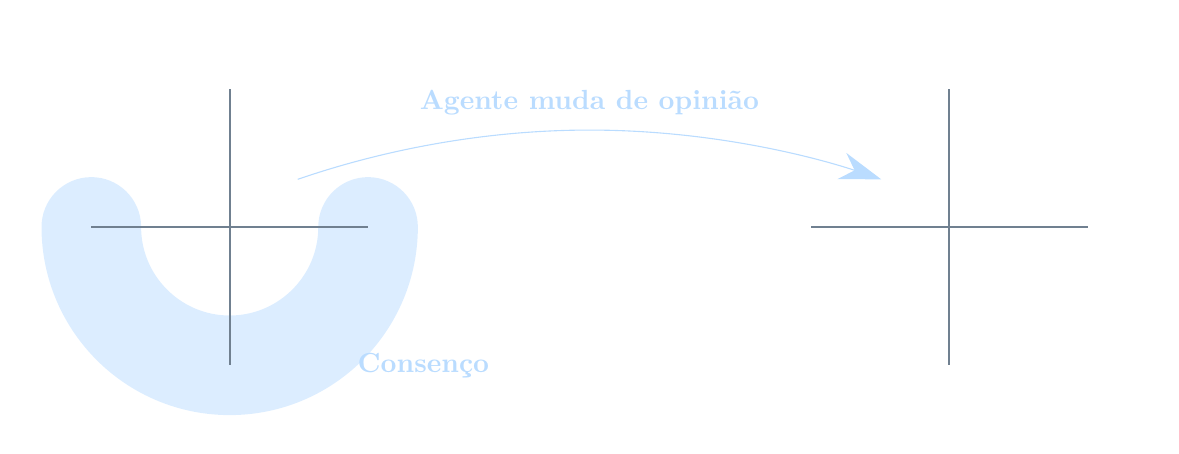
\begin{tikzpicture}[x=1em, y=1em]
\Canvas

\draw[gray, thick] (-13,0) -- (A1-east-agent);
\draw[gray, thick] (-13,0) -- (A1-west-agent);
\draw[gray, thick] (-13,0) -- (A1-north-agent);
\draw[gray, thick] (-13,0) -- (A1-south-agent);

\AgentMinus[(A1-center)]
\AgentPlus[(A1-east-agent)]
\AgentPlus[(A1-west-agent)]
\AgentMinus[(A1-north-agent)]
\AgentPlus[(A1-south-agent)]

\begin{scope}[shift={(-13,0)}, on background layer]
    \draw[LBlue, opacity=0.5, line cap=round, line join=round, line width=3.6em ] (A1-west-agent) arc ( -180:0:5 );
\end{scope}
\begin{scope}[shift={(-13,0)}]
    \node[text=LBlue, font=\bfseries] at ($(A1-east-agent)+(-90:5)+(2,0)$) {Consenço};
\end{scope}

\draw[gray, thick] (13,0) -- (A2-east-agent);
\draw[gray, thick] (13,0) -- (A2-west-agent);
\draw[gray, thick] (13,0) -- (A2-north-agent);
\draw[gray, thick] (13,0) -- (A2-south-agent);

\AgentPlus[(A2-center)]
\AgentPlus[(A2-east-agent)]
\AgentPlus[(A2-west-agent)]
\AgentMinus[(A2-north-agent)]
\AgentPlus[(A2-south-agent)]


\draw[LBlue,-{Stealth[length={1.5em}, width={1em}]}] ([shift={(35:3em)}]A1-center) parabola bend (0,3.5)  ([shift={(145:3em)}]A2-center);
\node[text=LBlue, font=\bfseries] at (0,4.5) {Agente muda de opinião};

\end{tikzpicture}

\begin{tikzpicture}[x=1em, y=1em]
\Canvas
\draw[gray, thick] (-13,0) -- (A1-east-agent);
\draw[gray, thick] (-13,0) -- (A1-west-agent);
\draw[gray, thick] (-13,0) -- (A1-north-agent);
\draw[gray, thick] (-13,0) -- (A1-south-agent);

\AgentMinus[(A1-center)]
\AgentPlus[(A1-east-agent)]
\AgentPlus[(A1-west-agent)]
\AgentMinus[(A1-north-agent)]
\AgentPlus[(A1-south-agent)]

\end{tikzpicture}


\begin{tikzpicture}[x=1em, y=1em]
\Canvas
\draw[gray, thick] (-13,0) -- (A1-east-agent);
\draw[gray, thick] (-13,0) -- (A1-west-agent);
\draw[gray, thick] (-13,0) -- (A1-north-agent);
\draw[gray, thick] (-13,0) -- (A1-south-agent);

\AgentMinus[(A1-center)]
\AgentPlus[(A1-east-agent)]
\AgentPlus[(A1-west-agent)]
\AgentMinus[(A1-north-agent)]
\AgentPlus[(A1-south-agent)]

\begin{scope}[shift={(-13,0)}, on background layer]
    \draw[LBlue, opacity=0.5, line cap=round, line join=round, line width=3.6em ] (A1-west-agent) arc ( -180:0:5 );
\end{scope}

\end{tikzpicture}

\begin{tikzpicture}[x=1em, y=1em]
\Canvas
\begin{scope}[shift={(-13,0)}]
    \node[text=LBlue, font=\bfseries] at ($(A1-east-agent)+(-90:5)+(2,0)$) {Consenço};
\end{scope}
\end{tikzpicture}


\begin{tikzpicture}[x=1em, y=1em]
\Canvas
\AgentPlus[(A2-center)]
\draw[LBlue,-{Stealth[length={1.5em}, width={1em}]}] ([shift={(35:3em)}]A1-center) parabola bend (0,3.5)  ([shift={(145:3em)}]A2-center);
\node[text=LBlue, font=\bfseries] at (0,4.5) {Agente muda de opinião};
\end{tikzpicture}

\begin{tikzpicture}[x=1em, y=1em]
\Canvas
\draw[gray, thick] (13,0) -- (A2-east-agent);
\draw[gray, thick] (13,0) -- (A2-west-agent);
\draw[gray, thick] (13,0) -- (A2-north-agent);
\draw[gray, thick] (13,0) -- (A2-south-agent);

\AgentPlus[(A2-center)]
\AgentPlus[(A2-east-agent)]
\AgentPlus[(A2-west-agent)]
\AgentMinus[(A2-north-agent)]
\AgentPlus[(A2-south-agent)]
\end{tikzpicture}

\end{document}